\chapter{Components}\label{ch:components}
\openepigraph{During human progress, every science is evolved out of its corresponding art.}{Herbert Spencer}
In LogicNet, every layer type has an implicit input Quantizer. The reason for this design choice is that input quantization is one of the most crucial aspects of an LogicNet, and output quantization is optional. The LUT cost increases linearly with the output bit-width of a neuron, whereas increases exponentially with the input fan-in bits. We lend the user some flexibility in output quantization, as it may be particularly important for the final layer. 
\section{Quantizer}
The Quantizer is a relatively simple module, which uses the Brevitas implementation of QuantHardTanh and QuantReLU. We can see clearly in \cref{fig:qhtanhqrelu} how QuantHardTanh and QuantReLU operate. The scaling factors are ignored so that we can discuss the bit-width with more ease.
If a bit-width of 1 is provided to the Quantizer, the class constructor initializes QuantHardTanh. If we provide a greater bit-width, we use a Quantized ReLU. For instance, if a bit-width of $3$ is provided, we can see that the QuantReLU will quantize any input to integer outputs from $0$ to $8$. This would also be then multiplied by a scaling factor. 
\begin{figure}[h]
    \centering
    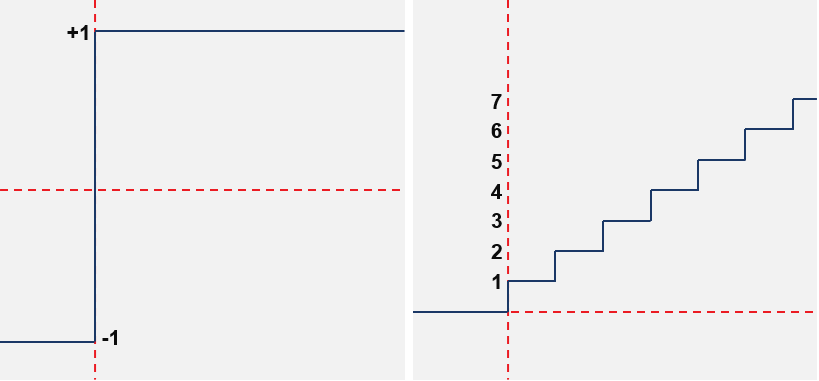
\includegraphics[width=300pt]{figures/bison/qhtanhqrelu.png}
    \caption{QuantHardTanh and QuantReLU Respectively. Scaling Factors not depicted.}
    \label{fig:qhtanhqrelu}
\end{figure}
    
The Quantizer returns a NamedTuple, which contains the Quantized Tensor in De-Quantized representation, with the scale-factor and the bit-width. Code Listing \ref{quantizeeg} depicts how a Quantizer operates on an input tensor.\\\\
\begin{lstlisting}[language=Python, caption=Example of a Quantizer, label=quantizeeg]
import torch
from LogicNet.quantizer import Quantizer
quantizer = Quantizer(bit_width = 1, max_val = 1.61)
print(quantizer(torch.randn(10)))
>>> QuantTensor(tensor=tensor([-1.6100, -1.6100, -1.6100,  
                1.6100, -1.6100, -1.6100, -1.6100,  1.6100,
                1.6100,  1.6100],
         grad_fn=<DifferentiableGraphBackward>),    
         scale=tensor(1.6100, grad_fn=<ClampMinBackward>), 
         bit_width=tensor(1.))
\end{lstlisting}

\section{SparseLinear}
The SparseLinear layer has an input Quantizer followed by a Linear Layer with a specific per-neuron fan in and Batch Normalization. The per-neuron fan-in is represented by a layer mask, and is initialized randomly when the layer is instantiated. It is important to note that in this implementation, the random sparsity is static and not learnable. For correct Truth Table generation, it expects us to give the next module in the forward pass. This is necessary to get the output bits a neuron produces for a specific input.

\newthoughtpar{LUTs}
The SparseLinear layer has a 'LUTS' attribute, that calculates the total number of LUTs that would be required when the class is instantiated. This functionality was added to aid design space exploration. The SparseLinear layer also has a method getLUTs() which returns the LUT cost of that layer.

\newthoughtpar{Truth Table Generation}
The SparseLinear layer has a generateTruthTable() method. Once called, it assigns an OrderedDict to the truthtable attribute of SparseLinear. This OrderedDict contains the TruthTable for each neuron.

\newthoughtpar{Truth Table functional verification}
The SparseLinear layer also supports forward pass which utilizes the TruthTable. This is important from a functional verification standpoint. The forward pass of the SparseLinear module has an argument 'use\_table', which when set allows forward pass through that layer using the truthtable dictionary.

\section{DenseQuantLinear}
The DenseQuantLinear layer has an Input Quantizer followed by a QuantLinear layer and Batch Normalization. 
\newthoughtpar{LUTs}
The DenseQuantLinear layer has a 'LUTS' attribute as well. The functionality is similar to SparseLinear, but the equation used is Equation \eqref{denseqlinlutformula}. In this formula, $n(O)$ and $n(I)$ refer to the output feature count and input feature count respectively. $BW_{in}$ and $BW_{wt}$ refer to the input bit-width and weight bit-width respectively. 
\begin{equation}
    LUTS = n(O)\times(n(I)\times BW_{in}\times BW_{wt}\times 1.0699 + 10.779)
    \label{denseqlinlutformula}
\end{equation}


\section{SparseConv}
Implementing Convolutions with a Sparsity that LogicNet can leverage is a tricky task. This is due to the fact that Convolutions typically have kernels with many channels, that are not independent. The LUT cost for a fully unfolded dense convolution is shown in Equation \eqref{lutcosteqn}. Where $outpix$ refers to the number of output pixels, $oBits$ refer to output bits, $n(OFM)$ refer to the number of output feature maps, $n(IFM)$ refers to the number of Input Feature Maps, $k$ refers to the kernel size (assuming square kernels) and $iBits$ refers to the number of Input bits.
\begin{equation}
    LUTs = outpix\times oBits \times n(OFM) * LUTCost(n(IFM)*k^{2}*iBits)
    \label{lutcosteqn}
\end{equation}

The most effective way we could find to deal with this is to introduce 'Depthwise Separable Convolutions' with Input and Intermediate Quantizers and Sparsity into the LogicNet library. \cref{fig:dwsepconv} depicts how such a Convolution would be implemented in the LogicNet library.\\

We give the user the ability to control the input bit-width, intermediate bit-width, as well as the sparsity of the Depthwise Kernels and Pointwise Kernels. The SparseConv also has Batch Normalization in both stages.
If the first\_layer argument is set true for SparseConv, it checks if the input channel count is 1. If that is true, it sets the Kernel count of Depthwise stage equal to the number of Output Feature Maps. This is useful because as the kernels are very sparse, it becomes harder to extract useful information out of the input image with just 1 randomly initialized sparse 2D kernel.

\begin{figure}[h]
    \centering
    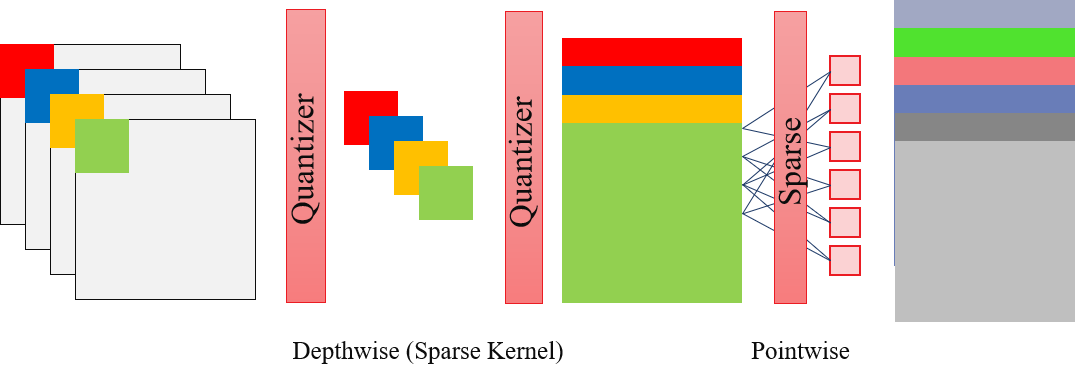
\includegraphics[width=300pt]{figures/bison/dwsepconv.png}
    \caption{Depthwise Separable Convolutions in LogicNet.}
    \label{fig:dwsepconv}
\end{figure}

\newthoughtpar{LUTs}
By virtue of using Depthwise-Separable Convolution, our LUT cost is divided to two parts. The Depthwise and Pointwise LUT cost.
Depthwise LUT Cost is given by Equation \eqref{dwLUTcost}. Here, $X_{k}$ refers to the Kernel Sparsity.
\begin{equation}
    LUTs_{dw} = outpix\times obits\times n(OFM)\times LUTcost(X_{k}\times ibits)
    \label{dwLUTcost}
\end{equation}
Pointwise LUT Cost is given by Equation \eqref{ptLUTcost}. Here, $X_{s}$ refers to the Pointwise Sparsity.
\begin{equation}
    LUTs_{pt} = outpix\times obits\times n(OFM)\times LUTcost(X_{s}\times ibits)
    \label{ptLUTcost}
\end{equation}

As this is a fully unfolded convolution, the LUT cost calculation requires the $outpix$ and $n(OFM)$. Thus, the LUTS attribute is populated only after a forward pass is done on the Model.
\newthoughtpar{Truth Table Generation}
The SparseConv layer has a generateTruthTable() method. Once called, it assigns an OrderedDict to the truthtable attribute of SparseConv. The OrderedDict contains separate OrderedDict for the Depthwise and Pointwise stages, with proper indexing for the neurons. 

\newthoughtpar{Truth Table Functional Verification}
The SparseConv layer also supports forward pass which utilizes the TruthTable. It is similar in nature to the SparseLinear. It is important to note that this is purely for Functional Verification, and is thus quite slow. It loops iteratively through every input window and uses the truth table for the forward pass. A vanilla convolution implementation had to be written to incorporate the forward pass with the Truth Table.

\begin{lstlisting}[language=Python, caption=Implementing Truth Table Functional Verification, label=convFuncVerif]
rlen = int(1 + (x.shape[-2] - self.kernel_size)/self.stride)
clen = int(1 + (x.shape[-1] - self.kernel_size)/self.stride)
dw_out = torch.zeros(x.shape[0], self.inWCout if (self.first_layer and self.inWCin==1) else self.inWCin, rlen, clen)        
for batch in range(x.shape[0]):
    for h in range(rlen):
        for w in range(clen):
            vert_start = h*self.stride
            vert_end = h*self.stride + self.kernel_size
            horiz_start = w*self.stride
            horiz_end = w*self.stride + self.kernel_size
            submatrix = x[batch, :, vert_start:vert_end, horiz_start:horiz_end]
            dw_out[batch, :, h, w] = lookupConvDW(self, self.truthtable['dw'], submatrix, (self.first_layer and self.inWCin==1))
\end{lstlisting}

% /*
% Introduction
% The need for accelerators
%     CPUs, GPUs, ASICs, FPGAs.
% Background
%     FPGA and HW/SW Co-Design
%     Mapping Neurons to Hardware
%       Sparsity
%           Expander, Iterative, Momentum
%       Quantize
%           Activation brevitas
%           Non Linear
% LogicNet: A Library for Mapping HBBs to NEQs
%     Introduction
%     Components
%       Linear
%       Convolutions
%     Design Automation
%       TruthTableGen
%       VerilogGen
%       Synthesis
% Testing LogicNet
%     LogicNet4HEP
%       Introduction
%       Models
%     MNIST 
%       Models
% Concluding Remarks
%     Research Questions
%     Conclusion
% */